\section{Introduction}
% State the problem, and its impact on all stakeholders (those directly affected, and society at large e.g. the social and economic impact of treating the disease)
A curvilinear structure in an image appears as a ribbon or bar of finite width that is distinguishable from the surrounding background, with a cross-sectional profile that is repeated along a linear, though not necessarily straight.

%What are their general characteristics?
%Defined locally by their cross-sectional profile and orientation, and assumed to extend in at least one direction normal to the profile (as opposed to a blob).

Detecting and measuring the properties of curvilinear structures in images is useful for many reasons~\cite{Ayres_Rangayyan_JEI07}:

\begin{itemize}
\item detecting distinctive patterns of vessels and fibrous tissue can improve quality of life and reduce costs associated with treating diseases such as retinopathy (\fref{f:first_pic}), diabetic neuropathy and breast cancer in advanced stages by aiding early diagnosis and treatment; %
\item spotting cracks and other similar defects in manufactured items such as roads, eggs can reduce costs associated with waste; %
\item biometrics based on ridge patterns in fingerprints~\cite{missing}, or the veins of the finger~\cite{missing} or hand~\cite{missing}, can bring criminals to justice and prevent further crime, or enhance the usability of technology by controlling access to sensitive data; %
\item detecting roads, railways and rivers in aerial photography can help to build maps automatically for applications such as providing relief in remote areas following a natural disaster.
\end{itemize}


\subsection{Aims and Objectives}

\begin{figure}[t]
\centering
\begin{tabular}{@{}c c c@{}}
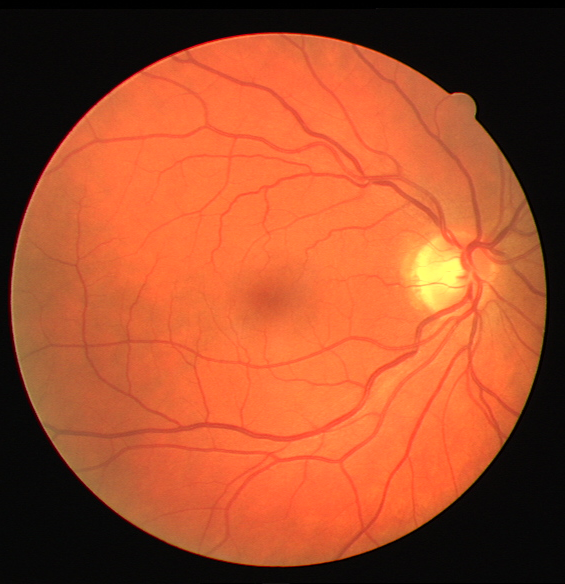
\includegraphics[width=0.3\columnwidth]{\figpath/retina/02_test} &
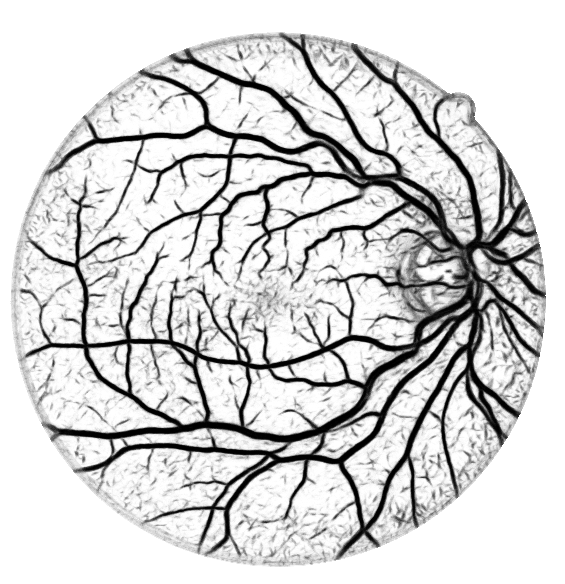
\includegraphics[width=0.3\columnwidth]{\figpath/retina/02_segmentation_gabor_inv.png} &
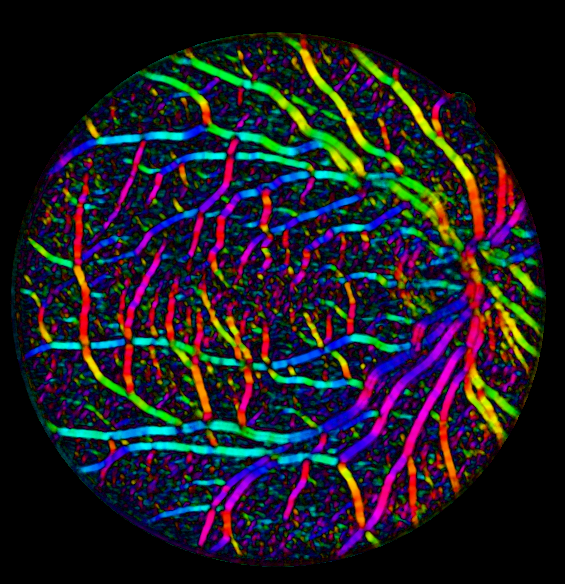
\includegraphics[width=0.3\columnwidth]{\figpath/retina/02_orientation_mag} \\
%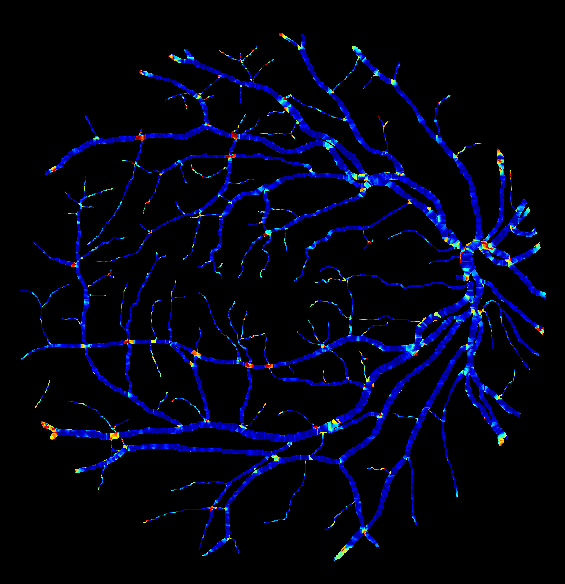
\includegraphics[height=0.15\textheight]{\figpath/retina/002_abs_error} \\
(a) & (b) & (c) \\
\noalign{\smallskip}
\end{tabular}
%
\caption{Estimating orientation in retinography: %
(a) input image; %
(b) segmentation of vessels by random forest classification of Gabor features; %
(c) orientation (indicated by colour) estimated using random regression over Gabor~features.}
\label{f:first_pic}
\end{figure}

% Specific aims of the study
Given an image, our aim is to determine where any linear structures exist in the image, and to measure values that correspond to low-level properties such as orientation, width, and cross-sectional profile. Although these properties form the basis of higher level, application-specific analysis (classifying structure as \emph{road}, \emph{rail} or \emph{river} in aerial photographs, for example), our focus is purely on computing the local attributes as accurately and robustly as possible; by improving the accuracy of the values we estimate, it follows logically that performance should improve for all higher level analysis methods that use these values as inputs.\footnote{Any algorithm that does not benefit from better input should be regarded with suspicion.}

%For example, any method to move from a map of vessel probabilities and predicted orientations in a retinograms, to an explicit grouping of pixels that belong to individual vessels, is likely to benefit from a priori knowledge of the spatial arrangement vessels in that image class and the physical model of how vessels grow and bifurcate. Such a method will therefore be very different from that needed to group a similar set of local information into the road, rivers etc present in an image for aerial analysis

With this focus, we have two objectives: extract, at every image location, structural information that is rich enough to capture the underlying image properties yet sparse enough to be computed efficiently; and combine this raw local information to predict output values of interest (such as orientation).


% Review other people's attempts at solving the problem, and why they are found wanting
\subsection{Related Work}
\comment{There is no 3D analogue of the \dtcwt{}. Therefore, we should avoid 3D datasets and related work as much as possible - this paper is solely about the analysis of 2D image structures. This includes aerial photography, retinal images, fingerprints and palmprints, surface inspection, and possibly fibre analysis.}

Because previous attempts at detecting and measuring curvilinear structures have been surveyed elsewhere, from the general~\cite{Papari_Petkov_IVC11} to the application-specific~\cite{Kirbas_Quek_ACMCS04,Lesage_etal_MIA09}, here we briefly review only a few papers in applications areas of specific interest. We will also discount the very basic detection methods that simply threshold an image~\cite{Jiang_Mojon_TPAMI03} and very complex methods that use techniques such as phase fields~\cite{Peng_etal_IJCV09}, leaving us free to focus on the most popular approaches that apply a bank of filters to the image before interpreting the responses in a way that accentuates the `lineness' at every pixel.

Early examples modelled a curvilinear structure as an image `ridge', typically defined using second order derivatives and formulated either as a Hessian problem~\cite{Frangi_etal_MICCAI98,Sato_etal_MIA98} or as responses to a derivative filter~\cite{Staal_etal_TMI04,Aylward_Bullitt_TMI02,Steger_TPAMI98,Koenderink_vanDoorn_TPAMI92}. Interpreting the responses to these filters used hand-crafted equations based on the differential geometry of the image `surface'~\cite{Frangi_etal_MICCAI98,Sato_etal_MIA98}.

With the maturing of machine learning, it was recognized that hand-crafting could be replaced by flexible statistical models whose parameters were optimized to agree with input-output training example pairs; Gaussian mixture models~\cite{Soares_etal_TMI06}, %
artificial neural networks~\cite{Marin_etal_TMI11,Minh_Hinton_ECCV10}, %
support vector machines~\cite{Ricci_Perfetti_TMI07,Gonzalez_etal_CVPR09}, and %
$k$-nearest neighbour classifiers~\cite{Staal_etal_TMI04} were all popular choices. Not only are these methods well-established and understood within machine learning, but a learnt statistical model can also accommodate different sensing modalities (with different noise properties) and other `stuff' that is hard to hand-craft, making the resulting algorithms more easily transferrable.

In addition, learnt statistical models can be applied to \emph{any} vector of image features to predict the quantity of interest, and are not tied to a particular feature type with specific theoretical properties. Furthermore, flexible statistical models permit the option to include hand-crafted, application-specific features where beneficial~\cite{Staal_etal_TMI04}. As a result, subsequent studies were free to use alternative filter banks and features based on %
matched filters or templates~\cite{Chaudhuri_etal_TMI89,Pechaud_etal_CVPR09,Dixon_Taylor_IPC79,Hoover_etal_TMI00,Ricci_Perfetti_TMI07}; %
derivatives of a first~\cite{Cai_Chung_MICCAI06} or higher than second~\cite{Gonzalez_etal_CVPR09} order; %
Gabor filters~\cite{Soares_etal_TMI06,Dabbah_etal_MIA11}; %
moments~\cite{Marin_etal_TMI11}; %
principal component analysis~\cite{Minh_Hinton_ECCV10}; %
wavelet transforms; %
and the monogenic signal. %
Some of these filter banks have been evaluated previously in a brief comparison~\cite{Ayres_Rangayyan_JEI07}, though the authors admit that not all filters were compared exactly on a like-for-like basis; our work builds on this comparison.

As well as permitting flexibility in the choice of input feature vector, learnt statistical predictors can be used to predict more than just the presence of a line. In recent studies, for example, orientation~\cite{Zwiggelaar_etal_TMI04,Ayres_Rangayyan_JEI07}, width~\cite{Steger_TPAMI98,Zwiggelaar_etal_TMI04} and multi-class labels~\cite{Zwiggelaar_etal_TMI04} have all been predicted from image feature vectors.

In this work, we are particularly interested in estimating orientation. At a low and intermediate level, orientation is important for steering computation~\cite{Sonka_99}, extracting profiles~\cite{Zwiggelaar_etal_TMI04,Staal_etal_TMI04}, grouping and tracking curvilinear features~\cite{Aylward_Bullitt_TMI02}, and directional filtering such as nonmaximal suppression and anisotropic diffusion~\cite{Perona_PAMI90}. Applications at a high level, however, are more diverse. \comment{This feels unfinished?}

Other facets of tube detection and measurement are interesting though not directly relevant to this work: %
detecting lines at multiple scales~\cite{Lindeberg_IJCV98,Sato_etal_MIA98}; %
dealing with junctions and bifurcations where multiple lines meet at a point~\cite{Chen_etal_TPAMI00};
regularizing estimated lines via snakes~\cite{Laptev_etal_MVA00} or dynamic programming~\cite{Gruen}; %
and line following or tracking~\cite{Aylward_Bullitt_TMI02,Perez_etal_ICCV01}.

\comment{ The paragraphs below have been shifted from elsewhere and are now somewhat homeless. Either rehouse, rewrite or delete...}

CLS orientation may be computed by assuming that it can be expressed as a (typically nonlinear) function of the responses to a given set of filters. Theoretically, we know this to be true for some filter banks (\eg~second derivatives of a Gaussian), though there are some complications.

First, when filters are applied at more than one scale we must ensure that we use the responses from the best scale for the true line width; analytic methods ~\cite{Karssemeijer_teBrake_TMI96,Mei_etal_IVC09} assume this is the scale with the greatest response, though this is not guaranteed in the presence of noise. Second, any analytic method that assumes noise to be additive and Gaussian may suffer when this is not the case; this is a particularly a risk in medical applications (\eg~ultrasound has multiplicative Rayleigh noise). Third, for some filter banks (such as the \dtcwt{}) an analytic solution is not well defined.

Our solution to these problems is to apply statistical methods that learn the association between input filter responses and an output orientation label over a set of training data.

Segmenting curvilinear structures such as blood vessels, ducts and nerve fibres in medical images is an important task, as shown by the extensive literature in the field~\cite{Papari_Petkov_IVC11,Staal_etal_TMI04,Ricci_Perfetti_TMI07}.


% Describe what we do, and why it is better than preceding works
\subsection{Our Contributions}
% Briefly outline our attempt at solving the problem, and why it should be better than the solutions that have preceded it
This paper presents three contributions that advance the current body of knowledge in the analysis of curvilinear image structures.

First, we provide a detailed comparison of commonly used image filter banks in the context of their suitability for extracting the local image information pertaining to curvilinear structure. In doing so, we describe the desirable properties of a suitable filter bank, therefore enabling us to make a principled choice that balances the richness of the extracted information against efficiency (both computational and storage). This analysis leads us to apply a previously unexploited image filter -- the dual-tree complex wavelet transform (\dtcwt{}) -- to the task of curvilinear feature analysis. The \dtcwt{} benefits from specific properties, such as efficiency and phase information, that address the shortcomings of existing popular image filters (\sref{s:filtering}).

Second, we investigate supervised learning approaches that, after training on a set of (input feature vector, target label) example pairs, turn a previously unseen feature vector of filter responses at a given location into an estimated output value. Specifically, we include the Random Forest statistical method to predict outputs, and compare this to techniques that have been previously used. For line detection (\ie~image segmentation), we show that a carefully selected filter bank, coupled with a modern learning method that is capable of dealing with non-linear data, produces results that match or exceed the state-of-the-art without relying on application-specific assumptions to boost performance. For orientation, we show how to formulate the learning problem such that angle wraparound is dealt with correctly, and in doing so produce \comment{significantly?} better estimates than existing methods that compute orientation analytically. In addition, we show how predicting output responses via machine learning allows us to estimate the error associated with the predictions, which we propose may in itself be of use in further processing.

Third, we explore the similarities and differences between these different approaches, and present empirical evidence of which work best in practice for real images including retinography and corneal confocal microscopy.

In all cases, we back up theoretical claims for filter performance with thorough experimental validation on both synthetic and real data.